\documentclass[
	classe=$1^{ere}STI2D$
]{évaluation}

\usepackage{diagbox}
\usepackage{tcolorbox}
\usetikzlibrary{calc}

\renewcommand{\arraystretch}{1.3}

\title{Évaluation : tableaux d'effectifs et de fréquences, probabilités}
\date{2 décembre 2022}
\author{}

\newcommand{\makeCorrection}{}
\newcommand{\Card}{\text{Card}}
\begin{document}

\maketitle

\begin{exercice} (sur le sujet)
	\begin{enumerate}
		\item \
		      \begin{center}
			      \begin{tabular}{|l|*{3}{>{\centering}p{2.2cm}|}}
				      \hline
				                  & fines  & épaisses & TOTAL \tabularnewline \hline
				      format $A3$ & $50$   & $125$    & $175$\tabularnewline \hline
				      format $A4$ & $750$  & $1150$   & $1900$ \tabularnewline \hline
				      format $A5$ & $200$  & $225$    & $425$ \tabularnewline \hline
				      TOTAL       & $1000$ & $1500$   & $2500$ \tabularnewline \hline
			      \end{tabular}
		      \end{center}
		\item Effectif des feuilles épaisses en format $A4$ : $1150$
		\item Pourcentage de feuilles $A3$ : $\frac{175}{2500} = 7\%$
	\end{enumerate}
\end{exercice}

\begin{exercice}\
	\begin{enumerate}
		\item \
		      \begin{center}
			      \begin{tabular}{|c|*{4}{>{\centering}p{1.5cm}|}}
				      \hline
				      \diagbox{$Y$}{$X$} & $x₁$  & $x₂$  & $x₃$  & TOTAL \tabularnewline \hline
				      $y₁$               & $164$ & $78$  & $80$  & $322$\tabularnewline \hline
				      $y₂$               & $36$  & $442$ & $200$ & $678$ \tabularnewline \hline
				      TOTAL              & $200$ & $520$ & $280$ & $1000$ \tabularnewline \hline
			      \end{tabular}
		      \end{center}
		\item \
		      \begin{center}
			      \begin{tabular}{|c|*{4}{>{\centering}p{1.5cm}|}}
				      \hline
				      \diagbox{$Y$}{$X$} & $x₁$     & $x₂$     & $x₃$   & TOTAL \tabularnewline \hline
				      $y₁$               & $16,4\%$ & $7,8\%$  & $8\%$  & $32,2\%$ \tabularnewline \hline
				      $y₂$               & $3,6\%$  & $44,2\%$ & $20\%$ & $67,8\%$ \tabularnewline \hline
				      TOTAL              & $20\%$   & $52\%$   & $28\%$ & $100\%$ \tabularnewline \hline
			      \end{tabular}
		      \end{center}
		\item $f_{12} = 7,8\%$ et $f_{23}= 20\%$.
		\item \
		      \begin{center}
			      \begin{tabular}{|c|*{1}{>{\centering}p{1.5cm}|}}
				      \hline
				      $Y$   & $x₁$     \tabularnewline \hline
				      $y₁$  & $82\%$ \tabularnewline \hline
				      $y₂$  & $18\%$  \tabularnewline \hline
				      TOTAL & $100\%$  \tabularnewline \hline
			      \end{tabular}
		      \end{center}
		\item \
		      \begin{center}
			      \begin{tabular}{|c|*{4}{>{\centering}p{1.5cm}|}}
				      \hline
				      $X$  & $x₁$    & $x₂$     & $x₃$     & TOTAL \tabularnewline \hline
				      $y₂$ & $5,3\%$ & $65,2\%$ & $29,5\%$ & $100\%$ \tabularnewline \hline
			      \end{tabular}
		      \end{center}
	\end{enumerate}
\end{exercice}

\begin{exercice} \

	\begin{enumerate}
		\item 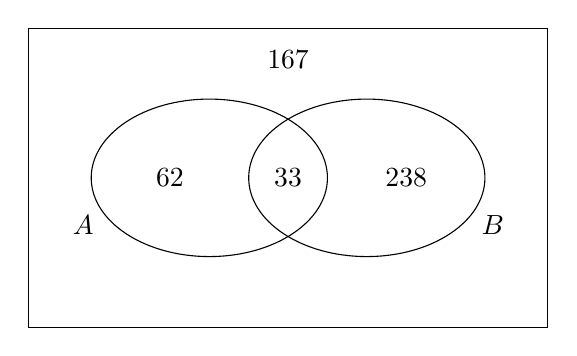
\begin{tikzpicture}
			      \coordinate (A) at (-1,0);
			      \coordinate (B) at (1,0);

			      \draw (-3.3,-1.9) rectangle (3.3,1.9);
			      \draw (A) ellipse (1.5 and 1);
			      \draw (B) ellipse (1.5 and 1);
			      \node at ($(A) + (-1.6,-0.6)$) {$A$};
			      \node at ($(B) + (1.6,-0.6)$) {$B$};

			      \node at ($(A) + (-0.5,0)$) {$62$};
			      \node at ($(0,0)$) {$33$};
			      \node at ($(0,1.5)$) {$167$};
			      \node at ($(B) + (0.5,0)$) {$238$};
		      \end{tikzpicture}
		\item $\Card(A ∩ B) = 33$
		\item $\Card(\overline{A} ∩ B) = 238$
		\item $\Card(A ∪ B) = 62+33+238=333$
		\item la probabilité qu'un passager soit en seconde classe ET qu'il n'ai pas mis ses bagages en soute s'écrit mathématiquement :

		      $P(\overline{A} ∩ \overline{B}) = \dfrac{167}{500} = 0,334$, soit $33,4\%$ de chances.
	\end{enumerate}
\end{exercice}

\begin{exercice} \

	\begin{enumerate}
		\item \
		      \begin{center}
			      \begin{tabular}{|l|*{3}{>{\centering}p{2cm}|}}
				      \hline
				      \diagbox{$X =$ fleur}{$Y =$ serre} & $A$        & $B$        & TOTAL \tabularnewline \hline
				      Tulipe                             & $88,2$ kg  & $163,8$ kg & $252$ kg\tabularnewline \hline
				      Narcisse                           & $19,6$ kg  & $78,4$ kg  & $98$ kg \tabularnewline \hline
				      TOTAL                              & $107,8$ kg & $242,2$ kg & $350$ kg \tabularnewline \hline
			      \end{tabular}
		      \end{center}
		\item $\dfrac{107,8}{350} = 30,8\%$ des fleurs proviennent de la serre A.
		\item Parmi les fleurs de la serre $B$, le pourcentage de tulipes est $\dfrac{163,8}{242,2} = 67,6\%$
	\end{enumerate}
\end{exercice}

\begin{exercice} \

	PAS DE SOLUTION ?
\end{exercice}

%======================
% SUJET B
%======================
\newpage
\setcounter{exercice}{1}

\maketitle

\begin{exercice} (sur le sujet)

	\begin{enumerate}
		\item \
		      \begin{center}
			      \begin{tabular}{|l|*{3}{>{\centering}p{2.2cm}|}}
				      \hline
				                  & fines & épaisses & TOTAL \tabularnewline \hline
				      format $A3$ & $40$  & $100$    & $140$ \tabularnewline \hline
				      format $A4$ & $600$ & $920$    & $1520$ \tabularnewline \hline
				      format $A5$ & $160$ & $180$    & $340$ \tabularnewline \hline
				      TOTAL       & $800$ & $1200$   & $2000$ \tabularnewline \hline
			      \end{tabular}
		      \end{center}
		\item Effectif des feuilles épaisses en format $A4$ : $920$
		\item Pourcentage de feuilles $A3$ : $\frac{140}{2000} = 7\%$
	\end{enumerate}
\end{exercice}

\begin{exercice}\
	\begin{enumerate}
		\item \
		      \begin{center}
			      \begin{tabular}{|c|*{4}{>{\centering}p{1.5cm}|}}
				      \hline
				      \diagbox{$Y$}{$X$} & $x₁$  & $x₂$  & $x₃$  & TOTAL \tabularnewline \hline
				      $y₁$               & $164$ & $78$  & $80$  & $322$\tabularnewline \hline
				      $y₂$               & $36$  & $442$ & $200$ & $678$ \tabularnewline \hline
				      TOTAL              & $200$ & $520$ & $280$ & $1000$ \tabularnewline \hline
			      \end{tabular}
		      \end{center}
		\item \
		      \begin{center}
			      \begin{tabular}{|c|*{4}{>{\centering}p{1.5cm}|}}
				      \hline
				      \diagbox{$Y$}{$X$} & $x₁$     & $x₂$     & $x₃$   & TOTAL \tabularnewline \hline
				      $y₁$               & $16,4\%$ & $7,8\%$  & $8\%$  & $32,2\%$ \tabularnewline \hline
				      $y₂$               & $3,6\%$  & $44,2\%$ & $20\%$ & $67,8\%$ \tabularnewline \hline
				      TOTAL              & $20\%$   & $52\%$   & $28\%$ & $100\%$ \tabularnewline \hline
			      \end{tabular}
		      \end{center}
		\item $f_{12} = 7,8\%$ et $f_{23}= 20\%$.
		\item \
		      \begin{center}
			      \begin{tabular}{|c|*{1}{>{\centering}p{1.5cm}|}}
				      \hline
				      $Y$   & $x₁$     \tabularnewline \hline
				      $y₁$  & $82\%$ \tabularnewline \hline
				      $y₂$  & $18\%$  \tabularnewline \hline
				      TOTAL & $100\%$  \tabularnewline \hline
			      \end{tabular}
		      \end{center}
		\item \
		      \begin{center}
			      \begin{tabular}{|c|*{4}{>{\centering}p{1.5cm}|}}
				      \hline
				      $X$  & $x₁$    & $x₂$     & $x₃$     & TOTAL \tabularnewline \hline
				      $y₂$ & $5,3\%$ & $65,2\%$ & $29,5\%$ & $100\%$ \tabularnewline \hline
			      \end{tabular}
		      \end{center}
	\end{enumerate}
\end{exercice}

\begin{exercice} \

	\begin{enumerate}
		\item 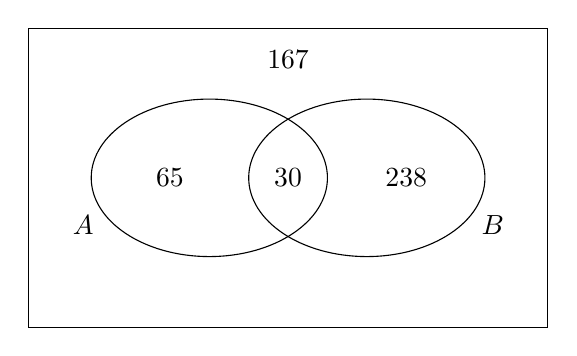
\begin{tikzpicture}
			      \coordinate (A) at (-1,0);
			      \coordinate (B) at (1,0);

			      \draw (-3.3,-1.9) rectangle (3.3,1.9);
			      \draw (A) ellipse (1.5 and 1);
			      \draw (B) ellipse (1.5 and 1);
			      \node at ($(A) + (-1.6,-0.6)$) {$A$};
			      \node at ($(B) + (1.6,-0.6)$) {$B$};

			      \node at ($(A) + (-0.5,0)$) {$65$};
			      \node at ($(0,0)$) {$30$};
			      \node at ($(0,1.5)$) {$167$};
			      \node at ($(B) + (0.5,0)$) {$238$};
		      \end{tikzpicture}
		\item $\Card(A ∩ B) = 30$
		\item $\Card(\overline{A} ∩ B) = 238$
		\item $\Card(A ∪ B) = 65+30+238=333$
		\item la probabilité qu'un passager soit en seconde classe ET qu'il n'ai pas mis ses bagages en soute s'écrit mathématiquement :

		      $P(\overline{A} ∩ \overline{B}) = \dfrac{167}{500} = 0,334$, soit $33,4\%$ de chances.
	\end{enumerate}
\end{exercice}

\begin{exercice} \

	\begin{enumerate}
		\item \
		      \begin{center}
			      \begin{tabular}{|l|*{3}{>{\centering}p{2cm}|}}
				      \hline
				      \diagbox{$X =$ fleur}{$Y =$ serre} & $A$        & $B$        & TOTAL \tabularnewline \hline
				      Tulipe                             & $88,2$ kg  & $163,8$ kg & $252$ kg \tabularnewline \hline
				      Narcisse                           & $19,6$ kg  & $78,4$ kg  & $98$ kg \tabularnewline \hline
				      TOTAL                              & $107,8$ kg & $242,2$ kg & $350$ kg \tabularnewline \hline
			      \end{tabular}
		      \end{center}
		\item $\dfrac{107,8}{350} = 30,8\%$ des fleurs proviennent de la serre A.
		\item Parmi les fleurs de la serre $B$, le pourcentage de tulipes est $\dfrac{163,8}{242,2} = 67,6\%$
	\end{enumerate}
\end{exercice}

\begin{exercice} \

	PAS DE SOLUTION ?
\end{exercice}

\end{document}